\section{Auswertung}
\label{sec:Auswertung}
\subsection{Bestimmung des magnetischen Moments die Schwingungsdauer}
Die für die Messung erhaltenen Werte befinden sich in Tabelle \ref{tab:schwing}.

\begin{table}[h]
  \label{tab:schwing}
    \centering
    \caption{Messwerte der Schwingung}
    \begin{tabular}{S[table-format=1.2(0)e0] S[table-format=2.1(0)e0] S[table-format=4.3(0)e0] S[table-format=1.3(0)e0] }
        \toprule
        {$I[\si{\ampere}]$} &       {$10\cdot T[\si{\second}]$} &       {$\frac{1}{B}[\si{1\per\tesla}]$} & {$T^2[\si{\second\squared}]$}\\
        \midrule
        0.50   & 19.84  & 1481.481  & 3.936\\
        1.00   & 14.68  &  740.741  & 2.155\\
        1.25   & 14.66  &  592.592  & 2.149\\
        1.50   & 12.12  &  493.827  & 1.468\\
        2.00   & 11.65  &  370.370  & 1.357\\
        2.50   & 10.37  &  296.296  & 1.075\\
        3.00   &  9.50  &  246.913  & 0.902\\
        3.25   &  9.03  &  227.920  & 0.815\\
        3.50   &  8.78  &  211.640  & 0.771\\
        4.00   &  8.25  &  185.185  & 0.681\\
        \bottomrule
    \end{tabular}
\end{table}
$T^2$ wird in Abbildung gegen $\frac{1}{B}$ aufgetragen.
Durch dieses Werte wird eine Gerade mittels linearer Regression aufgetragen.
\begin{figure}[H]
  \centering
  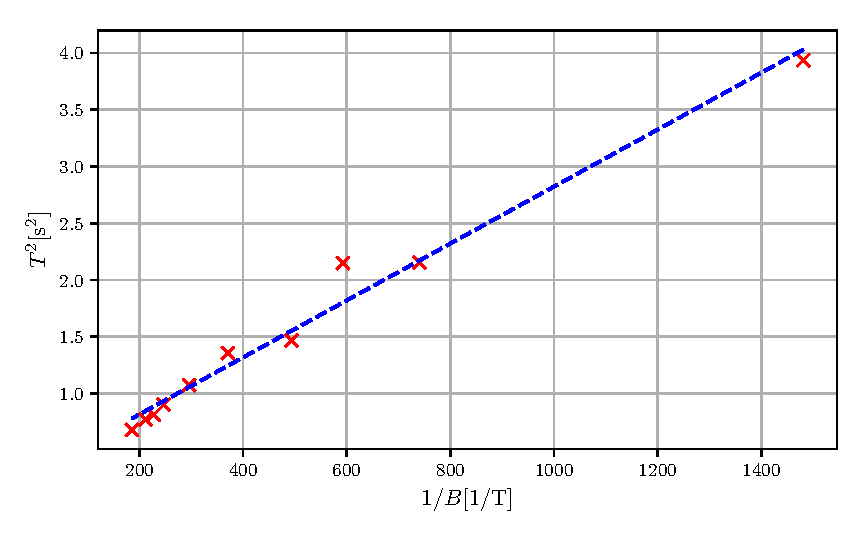
\includegraphics{schwing.pdf}
  \caption{Temperaturen der Wärmereservoirs aufgetragen gegen die Zeit.}
  \label{fig:schwing}
\end{figure}
Daraus folgt eine Steigung von $m=0.00251/pm 0.00012$ für die lineare Ausgleichsgerade.
Das magnetische Moment lässt sich dann nach Formel berechnen:
\begin{equation}
  \mu_{Dipol}= \frac{\pi^2 \cdot J_{Kugel}}{m}=(0.59)\si{\ampere\meter\squared}
\end{equation}
\subsection{Bestimmung des magnetischen Moments über Präzession}
